% Generated from the public primitive catalog. Original Atlas drawing; Apache-2.0.
% Target: slh-dsa-shake-192f; view: overview
\documentclass[border=9pt]{standalone}
% Original Atlas figure theme. Apache-2.0; see the repository LICENSE.
\usepackage[T1]{fontenc}
\usepackage{lmodern}
\usepackage{amsmath,amssymb}
\usepackage{tikz}
\usetikzlibrary{arrows.meta,positioning,calc,fit,backgrounds,decorations.pathreplacing,matrix}
\definecolor{atlasInk}{HTML}{172235}
\definecolor{atlasTeal}{HTML}{0D7B7D}
\definecolor{atlasMuted}{HTML}{637278}
\definecolor{atlasFill}{HTML}{EAF4F2}
\definecolor{atlasLine}{HTML}{B6C8C7}
\tikzset{
  every picture/.style={line width=.65pt,draw=atlasInk,>=Latex},
  every node/.style={text=atlasInk,font=\sffamily\small},
  box/.style={draw,rounded corners=1.5pt,minimum height=.9cm,minimum width=1.6cm,align=center,inner sep=6pt,fill=white},
  accent/.style={box,draw=atlasTeal,fill=atlasFill},
  wire/.style={->,line width=.7pt},
  keywire/.style={wire,draw=atlasTeal,dashed},
  xor/.style={draw,circle,fill=white,inner sep=0pt,minimum size=.38cm},
  add/.style={draw,rectangle,fill=white,inner sep=0pt,minimum size=.38cm},
  note/.style={font=\sffamily\scriptsize,text=atlasMuted,align=center},
  phase/.style={font=\sffamily\small\bfseries,text=atlasTeal},
  group/.style={draw=atlasLine,dashed,rounded corners=2pt,inner sep=8pt}
}
\newcommand{\rotl}{\mathbin{\lll}}
\newcommand{\rotr}{\mathbin{\ggg}}
\newcommand{\kx}{\operatorname{Keccak}\!\text{-}\!f[1600]}

\newcommand{\AtlasModulusBits}{b}
\newcommand{\AtlasFieldBits}{b}
\newcommand{\AtlasHash}{\textsf{H}}
\newcommand{\AtlasCurve}{\textsf{curve}}
\newcommand{\AtlasDhGroup}{\textsf{X25519 / X448}}
\newcommand{\AtlasDhPublicA}{\operatorname{XDH}(a,u_0)}
\newcommand{\AtlasDhPublicB}{\operatorname{XDH}(b,u_0)}
\newcommand{\AtlasDhSharedA}{\operatorname{XDH}(a,B)}
\newcommand{\AtlasDhSharedB}{\operatorname{XDH}(b,A)}
\newcommand{\AtlasSaltBytes}{s}
\newcommand{\AtlasSharedBits}{klen}
\newcommand{\AtlasPublicKeyBytes}{48}
\newcommand{\AtlasSecretKeyBytes}{96}
\newcommand{\AtlasCiphertextBytes}{|c|}
\newcommand{\AtlasSignatureBytes}{35664}
\newcommand{\AtlasModuleRank}{k}
\newcommand{\AtlasMatrixRows}{k}
\newcommand{\AtlasMatrixColumns}{\ell}
\newcommand{\AtlasHypertreeHeight}{66}
\newcommand{\AtlasHypertreeLayers}{22}
\newcommand{\AtlasForsHeight}{8}
\newcommand{\AtlasForsTrees}{33}
\newcommand{\AtlasHashBytes}{24}
\newcommand{\AtlasHashFamily}{\textsf{SHAKE}}
\begin{document}
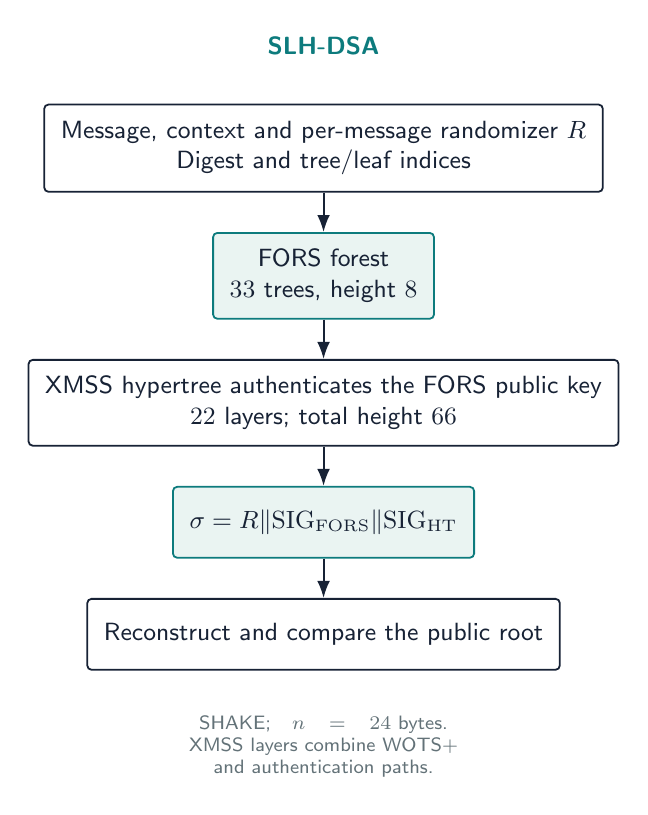
\begin{tikzpicture}[node distance=.5cm]
  \node[phase] (title) {SLH-DSA};
  \node[box,below=of title] (digest) {Message, context and per-message randomizer $R$\\Digest and tree/leaf indices};
  \node[accent,below=of digest] (fors) {FORS forest\\$\AtlasForsTrees$ trees, height $\AtlasForsHeight$};
  \node[box,below=of fors] (tree) {XMSS hypertree authenticates the FORS public key\\$\AtlasHypertreeLayers$ layers; total height $\AtlasHypertreeHeight$};
  \node[accent,below=of tree] (signature) {$\sigma=R\Vert\mathrm{SIG}_{\rm FORS}\Vert\mathrm{SIG}_{\rm HT}$};
  \node[box,below=of signature] (verify) {Reconstruct and compare the public root};
  \draw[wire] (digest) -- (fors); \draw[wire] (fors) -- (tree); \draw[wire] (tree) -- (signature); \draw[wire] (signature) -- (verify);
  \node[note,below=.45cm of verify,text width=6cm] {$\AtlasHashFamily$;\quad $n=\AtlasHashBytes$ bytes.\\XMSS layers combine WOTS+ and authentication paths.};
\end{tikzpicture}

\end{document}
